\subsection{Star\-List  Class Template Reference}
\label{class_starlist}\index{StarList@{Star\-List}}
lists of Stars. 


{\tt \#include $<$starlist.h$>$}

Inheritance diagram for Star\-List::\begin{figure}[H]
\begin{center}
\leavevmode
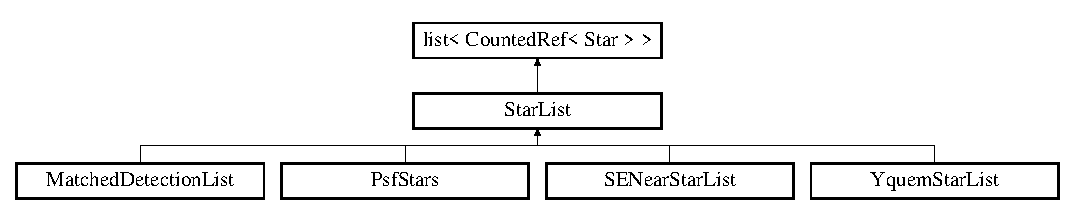
\includegraphics[height=2.44186cm]{class_starlist}
\end{center}
\end{figure}
\subsubsection*{Public Types}
\begin{CompactItemize}
\item 
\index{Element@{Element}!StarList@{Star\-List}}\index{StarList@{StarList}!Element@{Element}}
typedef {\bf Counted\-Ref}$<$Star$>$ {\bf Element}\label{class_starlist_s0}

\item 
\index{StarCIterator@{StarCIterator}!StarList@{Star\-List}}\index{StarList@{StarList}!StarCIterator@{Star\-CIterator}}
typedef list$<$Element$>$::const\_\-iterator {\bf Star\-CIterator}\label{class_starlist_s1}

\item 
\index{StarIterator@{StarIterator}!StarList@{Star\-List}}\index{StarList@{StarList}!StarIterator@{Star\-Iterator}}
typedef list$<$Element$>$::iterator {\bf Star\-Iterator}\label{class_starlist_s2}

\end{CompactItemize}
\subsubsection*{Public Methods}
\begin{CompactItemize}
\item 
\index{StarList@{StarList}!StarList@{Star\-List}}\index{StarList@{StarList}!StarList@{Star\-List}}
{\bf Star\-List} ()\label{class_starlist_a0}

\begin{CompactList}\small\item\em : default constructor (empty list).\item\end{CompactList}\item 
{\bf Star\-List} (const string \&File\-Name)
\begin{CompactList}\small\item\em reads a Star\-List from a file,.\item\end{CompactList}\item 
int {\bf write} (const string \&File\-Name)
\begin{CompactList}\small\item\em writes to a file.\item\end{CompactList}\item 
\index{read@{read}!StarList@{Star\-List}}\index{StarList@{StarList}!read@{read}}
int {\bf read} (const string \&File\-Name)\label{class_starlist_a3}

\begin{CompactList}\small\item\em obvious meaning.\item\end{CompactList}\item 
\index{push_back@{push\_\-back}!StarList@{Star\-List}}\index{StarList@{StarList}!push_back@{push\_\-back}}
void {\bf push\_\-back} (Star $\ast$t)\label{class_starlist_a4}

\item 
\index{push_back@{push\_\-back}!StarList@{Star\-List}}\index{StarList@{StarList}!push_back@{push\_\-back}}
void {\bf push\_\-back} (const Element \&e)\label{class_starlist_a5}

\item 
\index{~StarList@{$\sim$StarList}!StarList@{Star\-List}}\index{StarList@{StarList}!~StarList@{$\sim$Star\-List}}
virtual {\bf $\sim$Star\-List} ()\label{class_starlist_a6}

\item 
\index{dump@{dump}!StarList@{Star\-List}}\index{StarList@{StarList}!dump@{dump}}
void {\bf dump} (ostream \&stream=cout) const\label{class_starlist_a7}

\begin{CompactList}\small\item\em invokes dump(stream) for all Stars in the list.\item\end{CompactList}\item 
void {\bf Flux\-Sort} ()
\begin{CompactList}\small\item\em a model routine to sort the list.\item\end{CompactList}\item 
\index{ExtractHead@{ExtractHead}!StarList@{Star\-List}}\index{StarList@{StarList}!ExtractHead@{Extract\-Head}}
void {\bf Extract\-Head} (Star\-List$<$ Star $>$ \&Out, int NHead) const\label{class_starlist_a9}

\begin{CompactList}\small\item\em copy the head of the list at the end of an other list (that may be empty on input).\item\end{CompactList}\item 
\index{CutTail@{CutTail}!StarList@{Star\-List}}\index{StarList@{StarList}!CutTail@{Cut\-Tail}}
void {\bf Cut\-Tail} (const int NKeep)\label{class_starlist_a10}

\begin{CompactList}\small\item\em cuts the end of the list.\item\end{CompactList}\item 
\index{ExtractInFrame@{ExtractInFrame}!StarList@{Star\-List}}\index{StarList@{StarList}!ExtractInFrame@{Extract\-In\-Frame}}
void {\bf Extract\-In\-Frame} (Star\-List$<$ Star $>$ \&Out, const {\bf Frame} \&a\-Frame) const\label{class_starlist_a11}

\begin{CompactList}\small\item\em copy the part of the list which is included in the frame at the end of another list.\item\end{CompactList}\item 
\index{CutEdges@{CutEdges}!StarList@{Star\-List}}\index{StarList@{StarList}!CutEdges@{Cut\-Edges}}
void {\bf Cut\-Edges} (const {\bf Frame} \&a\-Frame, float mindist)\label{class_starlist_a12}

\begin{CompactList}\small\item\em cut the part of the list which is at a distance $<$ mindist of the edges defined by frame.\item\end{CompactList}\item 
\index{CopyTo@{CopyTo}!StarList@{Star\-List}}\index{StarList@{StarList}!CopyTo@{Copy\-To}}
void {\bf Copy\-To} (Star\-List$<$ Star $>$ \&Copy) const\label{class_starlist_a13}

\begin{CompactList}\small\item\em clears Copy and makes a copy of the list to Copy.\item\end{CompactList}\item 
\index{ClearList@{ClearList}!StarList@{Star\-List}}\index{StarList@{StarList}!ClearList@{Clear\-List}}
void {\bf Clear\-List} ()\label{class_starlist_a14}

\begin{CompactList}\small\item\em Clears the list.\item\end{CompactList}\item 
template$<$class Operator$>$ void {\bf Apply\-Transfo} (const Operator \&Op)
\begin{CompactList}\small\item\em enables to apply a geometrical transfo if Star is Basestar or derives from it.\item\end{CompactList}\item 
\index{FindClosest@{FindClosest}!StarList@{Star\-List}}\index{StarList@{StarList}!FindClosest@{Find\-Closest}}
Star$\ast$ {\bf Find\-Closest} (double X, double Y) const\label{class_starlist_a16}

\begin{CompactList}\small\item\em returns the closest Star from a given location.\item\end{CompactList}\item 
\index{FindClosest@{FindClosest}!StarList@{Star\-List}}\index{StarList@{StarList}!FindClosest@{Find\-Closest}}
Star$\ast$ {\bf Find\-Closest} (const {\bf Point} \&P) const\label{class_starlist_a17}

\begin{CompactList}\small\item\em same as above. Can be used with any of our star-like stuff.\item\end{CompactList}\item 
\index{HasCloseNeighbor@{HasCloseNeighbor}!StarList@{Star\-List}}\index{StarList@{StarList}!HasCloseNeighbor@{Has\-Close\-Neighbor}}
bool {\bf Has\-Close\-Neighbor} (double X, double Y, double maxdist, double mindist=0.1) const\label{class_starlist_a18}

\begin{CompactList}\small\item\em true if location has a nearby star in a ring between mindist and maxdist.\item\end{CompactList}\item 
\index{HasCloseNeighbor@{HasCloseNeighbor}!StarList@{Star\-List}}\index{StarList@{StarList}!HasCloseNeighbor@{Has\-Close\-Neighbor}}
bool {\bf Has\-Close\-Neighbor} (const {\bf Point} \&P, double maxdist, double mindist=0.1) const\label{class_starlist_a19}

\begin{CompactList}\small\item\em same as above. Can be used with any of our star-like stuff.\item\end{CompactList}\item 
\index{ClosestNeighbor@{ClosestNeighbor}!StarList@{Star\-List}}\index{StarList@{StarList}!ClosestNeighbor@{Closest\-Neighbor}}
Star$\ast$ {\bf Closest\-Neighbor} (double X, double Y, double mindist=0.1) const\label{class_starlist_a20}

\begin{CompactList}\small\item\em nearby star to a star but not itself.\item\end{CompactList}\item 
\index{ClosestNeighbor@{ClosestNeighbor}!StarList@{Star\-List}}\index{StarList@{StarList}!ClosestNeighbor@{Closest\-Neighbor}}
Star$\ast$ {\bf Closest\-Neighbor} (const {\bf Point} \&P, double mindist=0.1) const\label{class_starlist_a21}

\begin{CompactList}\small\item\em same as above. Can be used with any of our star-like stuff.\item\end{CompactList}\item 
\index{NumberOfNeighbors@{NumberOfNeighbors}!StarList@{Star\-List}}\index{StarList@{StarList}!NumberOfNeighbors@{Number\-Of\-Neighbors}}
int {\bf Number\-Of\-Neighbors} (const double \&X, const double \&Y, const double \&distmax) const\label{class_starlist_a22}

\item 
\index{AllNeighbors@{AllNeighbors}!StarList@{Star\-List}}\index{StarList@{StarList}!AllNeighbors@{All\-Neighbors}}
int {\bf All\-Neighbors} (Star\-List \&Neighbor\-List, const double \&X, const double \&Y, const double \&distmax) const\label{class_starlist_a23}

\item 
\index{AllNeighbors@{AllNeighbors}!StarList@{Star\-List}}\index{StarList@{StarList}!AllNeighbors@{All\-Neighbors}}
int {\bf All\-Neighbors} (Star\-List \&Neighbor\-List, const {\bf Point} \&Pt, const double \&distmax) const\label{class_starlist_a24}

\item 
\index{NumberOfNeighbors@{NumberOfNeighbors}!StarList@{Star\-List}}\index{StarList@{StarList}!NumberOfNeighbors@{Number\-Of\-Neighbors}}
int {\bf Number\-Of\-Neighbors} (const {\bf Point} \&Pt, const double \&distmax) const\label{class_starlist_a25}

\end{CompactItemize}
\subsubsection*{Protected Methods}
\begin{CompactItemize}
\item 
\index{ascii_read@{ascii\_\-read}!StarList@{Star\-List}}\index{StarList@{StarList}!ascii_read@{ascii\_\-read}}
int {\bf ascii\_\-read} (const string \&File\-Name)\label{class_starlist_b0}

\end{CompactItemize}


\subsubsection{Detailed Description}
\subsubsection*{template$<$class Star$>$  class Star\-List}

lists of Stars.

It is a template class, which means that the Star type remains undefined until a user defines it.  The list related operations (insertion, sort, traversal) are to be carried out using STL  list operations. Most of the Star operations rely on routines to be provided in  the Star class, usually user defined. The instanciation of this class for  {\bf Base\-Star} {\rm (p.\,\pageref{class_basestar})} (i.e. the replacement  of the formal parameter 'Star' by '{\bf Base\-Star} {\rm (p.\,\pageref{class_basestar})}') is  called Base\-Star\-List.  Take care: what is stored is pointers on Star's and  NOT Star's. This implies that Stars being inserted in the list have to be  obtained using 'new'. The corresponding 'delete' are invoked in the destructor. 



\subsubsection{Constructor \& Destructor Documentation}
\index{StarList@{Star\-List}!StarList@{StarList}}
\index{StarList@{StarList}!StarList@{Star\-List}}
\paragraph{\setlength{\rightskip}{0pt plus 5cm}template$<$class Star$>$ Star\-List$<$Star$>$::Star\-List$<$Star$>$ (const string \& {\em File\-Name})}\hfill\label{class_starlist_a1}


reads a Star\-List from a file,.

using the read method from the Star class.  See {\bf Base\-Star} {\rm (p.\,\pageref{class_basestar})} for an example of implementation. 

\subsubsection{Member Function Documentation}
\index{StarList@{Star\-List}!ApplyTransfo@{ApplyTransfo}}
\index{ApplyTransfo@{ApplyTransfo}!StarList@{Star\-List}}
\paragraph{\setlength{\rightskip}{0pt plus 5cm}template$<$class Star$>$  template$<$class Operator$>$ void Star\-List$<$Star$>$::Apply\-Transfo (const Operator \& {\em Op})\hspace{0.3cm}{\tt  [inline]}}\hfill\label{class_starlist_a15}


enables to apply a geometrical transfo if Star is Basestar or derives from it.

could be extended to other type of transformations. \index{StarList@{Star\-List}!FluxSort@{FluxSort}}
\index{FluxSort@{FluxSort}!StarList@{Star\-List}}
\paragraph{\setlength{\rightskip}{0pt plus 5cm}template$<$class Star$>$ void Star\-List$<$Star$>$::Flux\-Sort ()\hspace{0.3cm}{\tt  [inline]}}\hfill\label{class_starlist_a8}


a model routine to sort the list.

see {\bf Decreasing\-Flux}() {\rm (p.\,\pageref{basestar_h_a7})} to see what it is, if you  want another sorting criterion) \index{StarList@{Star\-List}!write@{write}}
\index{write@{write}!StarList@{Star\-List}}
\paragraph{\setlength{\rightskip}{0pt plus 5cm}template$<$class Star$>$ int Star\-List$<$Star$>$::write (const string \& {\em File\-Name})}\hfill\label{class_starlist_a2}


writes to a file.

calls iteratively the write method of the Star  class. It is unusable if the Star class does not  provide this functionnality. see {\bf Base\-Star} {\rm (p.\,\pageref{class_basestar})} to see a possible implementation.  not const because the write routines of Root are not 

The documentation for this class was generated from the following file:\begin{CompactItemize}
\item 
{\bf starlist.h}\end{CompactItemize}
